\documentclass[12pt,a4paper]{article}
\usepackage[utf8]{vietnam}
\usepackage{amsmath,amssymb}
\usepackage{geometry}
\geometry{top=1.5cm,bottom=1.2cm,left=1.4cm,right=1.4cm,headheight=28pt,headsep=12pt,footskip=18pt}
\usepackage{tikz}
\usepackage{xcolor}
\usepackage{enumerate}
\usepackage{graphicx}
\usepackage[version=4]{mhchem}
\usepackage{fancyhdr}
\usepackage{ex_test}

\renewcommand{\baselinestretch}{0.96}
\setlength{\parskip}{0pt}

\definecolor{hfRed}{RGB}{211,47,47}
\definecolor{hfGreen}{RGB}{139,195,144}

\pagestyle{fancy}
\fancyhf{}
\fancyhead[L]{\small\itshape\color{hfRed} Tài liệu lưu hành nội bộ}
\fancyhead[R]{\small\itshape\color{hfRed} Thầy \textbf{TRẦN VĂN THẠNH} - 0777.470.803}
\renewcommand{\headrulewidth}{0.8pt}
\renewcommand{\headrule}{\hbox to\headwidth{\color{hfGreen}\leaders\hrule height \headrulewidth\hfill}}

\fancyfoot[L]{\small\itshape\color{hfRed} CS1: 6/15 Nguyễn Hoàng, P. Kim Long, TP Huế \quad|\quad CS2: 24 Đặng Thái Thân, TP Huế}
\fancyfoot[R]{\small\bfseries\color{hfRed} Trang \thepage}
\renewcommand{\footrulewidth}{0.8pt}
\renewcommand{\footrule}{\hbox to\headwidth{\color{hfGreen}\leaders\hrule height \footrulewidth\hfill}}

\fancypagestyle{firstpage}{
  \fancyhf{}
  \renewcommand{\headrulewidth}{0pt}
  \fancyfoot[L]{\small\itshape\color{hfRed} CS1: 6/15 Nguyễn Hoàng, P. Kim Long, TP Huế \quad|\quad CS2: 24 Đặng Thái Thân, TP Huế}
  \fancyfoot[R]{\small\bfseries\color{hfRed} Trang \thepage}
  \renewcommand{\footrulewidth}{0.8pt}
  \renewcommand{\footrule}{\hbox to\headwidth{\color{hfGreen}\leaders\hrule height \footrulewidth\hfill}}
}

\begin{document}
\thispagestyle{firstpage}

\noindent
\begin{minipage}[t]{0.44\textwidth}
	\centering\fontsize{10pt}{12pt}\selectfont
	\textbf{SỞ GIÁO DỤC VÀ ĐÀO TẠO THỪA THIÊN HUẾ}\\
	\textbf{ĐỀ CHÍNH THỨC}\\
	\textit{(Đề thi có 04 trang)}
\end{minipage}\hfill
\begin{minipage}[t]{0.54\textwidth}
	\centering\small
	\textbf{ĐỀ KIỂM TRA ĐỊNH KỲ CHƯƠNG 1 (CÂN BẰNG HÓA HỌC)}\\
	\textbf{MÔN: HOÁ HỌC -- LỚP 11}\\
	\textit{Thời gian làm bài: 45 phút (không kể thời gian phát đề)}\\
	\fbox{\textbf{MÃ ĐỀ: 103}}
\end{minipage}

\smallskip
\noindent\hrulefill
\smallskip

\noindent\textbf{Họ, tên thí sinh:} \dotfill\ \textbf{Lớp:} \dotfill\ \textbf{Số báo danh:} \dotfill

\smallskip
\noindent\textit{(Cho biết nguyên tử khối: H = 1; C = 12; N = 14; O = 16; Na = 23; Al = 27; P = 31; S = 32; Cl = 35,5; K = 39; Ca = 40; I = 127; Ba = 137).}
\smallskip

\noindent
\textbf{PHẦN I (4,5 điểm -- 18 câu): Câu trắc nghiệm nhiều phương án lựa chọn.}\\
\textit{Thí sinh trả lời từ câu 1 đến câu 18. Mỗi câu hỏi thí sinh chỉ chọn một phương án.}

\Opensolutionfile{ans}[ans-hoa11-de03hs]

\begin{ex}
Cho cân bằng hoá học: $\ce{H2(g) + I2(g) <=> 2HI(g)} \quad \Delta_r H^\circ_{298} > 0$. Cân bằng không bị chuyển dịch khi
\choice
{Tăng nhiệt độ của hệ.}
{Giảm nồng độ $\ce{HI}$.}
{Tăng nồng độ $\ce{H2}$.}
{Giảm áp suất chung của hệ.}
\loigiai{}
\end{ex}

\begin{ex}
Cho cân bằng hóa học: $\ce{N2(g) + 3H2(g) <=> 2NH3(g)}$. Phản ứng thuận là phản ứng tỏa nhiệt. Cân bằng hóa học không bị dịch chuyển khi
\choice
{Thay đổi áp suất của hệ.}
{Thay đổi nồng độ $\ce{N2}$.}
{Thay đổi nhiệt độ.}
{Thêm chất xúc tác.}
\loigiai{}
\end{ex}

\begin{ex}
Cho cân bằng hoá học: $\ce{2SO2(g) + O2(g) <=> 2SO3(g)}$; phản ứng thuận là phản ứng tỏa nhiệt. Phát biểu đúng là:
\choice
{Cân bằng chuyển dịch theo chiều thuận khi tăng nhiệt độ.}
{Cân bằng chuyển dịch theo chiều nghịch khi giảm nồng độ $\ce{O2}$.}
{Cân bằng chuyển dịch theo chiều thuận khi giảm áp suất hệ phản ứng.}
{Cân bằng chuyển dịch theo chiều nghịch khi giảm nồng độ $\ce{SO3}$.}
\loigiai{}
\end{ex}

\begin{ex}
Các yếu tố ảnh hưởng đến cân bằng hoá học là
\choice
{Nồng độ, nhiệt độ và chất xúc tác.}
{Nồng độ, áp suất và diện tích bề mặt.}
{Nồng độ, nhiệt độ và áp suất.}
{Áp suất, nhiệt độ và chất xúc tác.}
\loigiai{}
\end{ex}

\begin{ex}
Dãy các chất gồm những chất điện li mạnh là:
\choice
{$\ce{NaF, NaOH, KCl, BaCl2}$}
{$\ce{HCl, NaCl, Na2CO3, Hg(CN)2}$}
{$\ce{KNO3, MgCl2, HNO3, HF}$}
{$\ce{NaOH, KCl, H2SO4, KOH, HClO}$}
\loigiai{}
\end{ex}

\begin{ex}
Nhúng giấy quỳ vào dung dịch có $\text{pH} = 4$ giấy quỳ chuyển thành màu:
\choice
{Đỏ}
{Xanh}
{Không đổi màu}
{Chưa xác định được}
\loigiai{}
\end{ex}

\begin{ex}
Dung dịch chất nào sau đây làm quỳ tím chuyển thành màu đỏ?
\choice
{$\ce{H2SO4}$.}
{$\ce{KOH}$.}
{$\ce{NaCl}$.}
{$\ce{C2H5OH}$.}
\loigiai{}
\end{ex}

\begin{ex}
Dung dịch của một base ở $25^\circ\text{C}$ có:
\choice
{$[\ce{H+}] = 1{,}0 \cdot 10^{-7}\text{ M}$}
{$[\ce{H+}] < 1{,}0 \cdot 10^{-7}\text{ M}$}
{$[\ce{H+}] > 1{,}0 \cdot 10^{-7}\text{ M}$}
{$[\ce{H+}][\ce{OH-}] > 1{,}0 \cdot 10^{-14}$}
\loigiai{}
\end{ex}

\begin{ex}
Dung dịch acid mạnh $\ce{H2SO4}\ 0{,}10\text{M}$ có:
\choice
{$\text{pH} = 1{,}00$}
{$\text{pH} < 1{,}00$}
{$\text{pH} > 1{,}00$}
{$[\ce{H+}] > 0{,}20\text{M}$}
\loigiai{}
\end{ex}

\begin{ex}
Xét các hệ cân bằng sau đây trong một bình kín:
\begin{enumerate}[(1)]
	\item $\ce{2NaHCO3(s) <=> Na2CO3(s) + H2O(g) + CO2(g)}$
	\item $\ce{CO2(g) + CaO(s) <=> CaCO3(s)}$
	\item $\ce{C(s) + CO2(g) <=> 2CO(g)}$
	\item $\ce{CO(g) + H2O(g) <=> CO2(g) + H2(g)}$
\end{enumerate}
Khi thêm $\ce{CO2}$ vào hệ thì số cân bằng chuyển dịch theo chiều thuận là
\choice
{2.}
{1.}
{4.}
{3.}
\loigiai{}
\end{ex}

\begin{ex}
Cho cân bằng hoá học sau: $\ce{2NH3(g) <=> N2(g) + 3H2(g)}$. Khi tăng nhiệt độ của hệ thì tỉ khối của hỗn hợp so với hydrogen giảm. Nhận xét nào sau đây là đúng?
\choice
{Khi tăng nhiệt độ của hệ, cân bằng chuyển dịch theo chiều thuận.}
{Phản ứng thuận là phản ứng toả nhiệt.}
{Khi tăng áp suất của hệ, cân bằng chuyển dịch theo chiều thuận.}
{Khi tăng nồng độ của $\ce{NH3}$, cân bằng chuyển dịch theo chiều nghịch.}
\loigiai{}
\end{ex}

\begin{ex}
Sự dịch chuyển cân bằng hoá học là sự di chuyển từ trạng thái cân bằng hoá học này
\choice
{Sang trạng thái cân bằng hóa học khác không cần có tác động của các yếu tố từ bên ngoài tác động lên cân bằng.}
{Sang trạng thái không cân bằng do tác động của các yếu tố từ bên ngoài tác động lên cân bằng.}
{Sang trạng thái cân bằng hoá học khác do tác động của các yếu tố từ bên ngoài tác động lên cân bằng.}
{Sang trạng thái cân bằng hoá học khác do cân bằng hóa học tác động lên các yếu tố bên ngoài.}
\loigiai{}
\end{ex}

\begin{ex}
\textbf{(SBT - KNTT)} Cho phản ứng hoá học sau: $\ce{PCl3(g) + Cl2(g) <=> PCl5(g)}$ ở $T^\circ\text{C}$, nồng độ các chất ở trạng thái cân bằng như sau: $[\ce{PCl5}] = 0{,}059\text{ mol/L}$; $[\ce{PCl3}] = [\ce{Cl2}] = 0{,}035\text{ mol/L}$. Hằng số cân bằng ($K_C$) của phản ứng tại $T^\circ\text{C}$ là
\choice
{$1{,}68.$}
{$48{,}16.$}
{$0{,}02.$}
{$16{,}95.$}
\loigiai{}
\end{ex}

\begin{ex}
Trong một bình kín có cân bằng hóa học sau: $\ce{2NO2(g) <=> N2O4(g)}$. Tỉ khối hơi của hỗn hợp khí trong bình so với $\ce{H2}$ ở nhiệt độ $T_1$ bằng $27{,}6$ và ở nhiệt độ $T_2$ bằng $34{,}5$. Biết $T_1 > T_2$. Phát biểu nào sau đây về cân bằng trên là đúng?
\choice
{Phản ứng thuận là phản ứng tỏa nhiệt.}
{Khi tăng nhiệt độ, áp suất chung của hệ cân bằng giảm.}
{Khi giảm nhiệt độ, áp suất chung của hệ cân bằng tăng.}
{Phản ứng nghịch là phản ứng tỏa nhiệt.}
\loigiai{}
\end{ex}

\begin{ex}
Khi hoà tan $\ce{SO2}$ vào nước có cân bằng sau: $\ce{SO2 + H2O <=> HSO3- + H+}$. Khi cho thêm $\ce{NaOH}$ và khi cho thêm $\ce{H2SO4}$ loãng vào dung dịch trên thì cân bằng sẽ chuyển dịch tương ứng là
\choice
{Thuận và thuận.}
{Thuận và nghịch.}
{Nghịch và thuận.}
{Nghịch và nghịch.}
\loigiai{}
\end{ex}

\begin{ex}
Cho các cân bằng sau:
\begin{enumerate}[(1)]
	\item $\ce{N2(g) + 3H2(g) <=> 2NH3(g)}$
	\item $\ce{H2(g) + I2(g) <=> 2HI(g)}$
	\item $\ce{CaCO3(s) <=> CaO(s) + CO2(g)}$
\end{enumerate}
Khi tăng áp suất chung của hệ thì cân bằng:
\choice
{(1) và (3) dịch chuyển theo chiều thuận; (2) không dịch chuyển.}
{(1) dịch chuyển theo chiều thuận; (2) không dịch chuyển; (3) dịch chuyển theo chiều nghịch.}
{(1) và (3) dịch chuyển theo chiều nghịch; (2) không dịch chuyển.}
{(1) dịch chuyển theo chiều nghịch; (2) không dịch chuyển; (3) dịch chuyển theo chiều thuận.}
\loigiai{}
\end{ex}

\begin{ex}
Trộn hai thể tích bằng nhau của dung dịch $\ce{H2SO4}$ và dung dịch $\ce{NaOH}$ có cùng nồng độ mol, pH của dung dịch sau phản ứng sẽ như thế nào?
\choice
{$\text{pH} = 7$}
{$\text{pH} > 7$}
{$\text{pH} < 7$}
{Không xác định được}
\loigiai{}
\end{ex}

\begin{ex}
Cho phản ứng: $\ce{H2(g) + I2(g) <=> 2HI(g)}$. Ở nhiệt độ $430^\circ\text{C}$, hằng số cân bằng $K_C$ của phản ứng trên bằng $53{,}96$. Đun nóng một bình kín dung tích không đổi 10 lít chứa $4{,}0\text{ gam } \ce{H2}$ và $406{,}4\text{ gam } \ce{I2}$. Khi hệ phản ứng đạt trạng thái cân bằng ở $430^\circ\text{C}$, nồng độ của $\ce{HI}$ là
\choice
{$0{,}275\text{M}.$}
{$0{,}225\text{M}.$}
{$0{,}151\text{M}.$}
{$0{,}320\text{M}.$}
\loigiai{}
\end{ex}

\Closesolutionfile{ans}

\bigskip
\noindent
\textbf{PHẦN II (4,0 điểm -- 4 câu): Câu trắc nghiệm đúng sai.}\\
\textit{Thí sinh trả lời từ câu 1 đến câu 4. Trong mỗi ý a), b), c), d) ở mỗi câu, thí sinh chọn đúng hoặc sai.}

\begin{ex}
Cho các phát biểu sau về trạng thái cân bằng hóa học:
\choiceTF
{Ở trạng thái cân bằng, tốc độ phản ứng thuận bằng tốc độ phản ứng nghịch.}
{Ở trạng thái cân bằng, các chất không phản ứng với nhau.}
{Ở trạng thái cân bằng, nồng độ các chất sản phẩm luôn lớn hơn nồng độ các chất đầu.}
{Ở trạng thái cân bằng, nồng độ các chất không thay đổi.}
\loigiai{}
\end{ex}

\begin{ex}
Khi hoà tan khí chlorine vào nước tạo thành dung dịch có màu vàng nhạt gọi là nước chlorine. Trong nước chlorine xảy ra cân bằng hoá học sau:
\[\ce{Cl2 + H2O <=> HClO + HCl \quad (1)}\]
Acid $\ce{HClO}$ sinh ra không bền, dễ bị phân huỷ theo phản ứng:
\[\ce{HClO -> HCl + O \quad (2)}\]
\choiceTF
{Nước chlorine sẽ nhạt màu dần theo thời gian, không bảo quản được lâu.}
{Phản ứng phân huỷ acid $\ce{HClO}$ làm giảm nồng độ của chất này, cân bằng (1) chuyển dịch theo chiều thuận.}
{Nước chlorine sẽ đậm màu dần theo thời gian, nên bảo quản được lâu.}
{Phản ứng phân huỷ acid $\ce{HClO}$ làm tăng nồng độ của chất này, cân bằng (1) chuyển dịch theo chiều nghịch.}
\loigiai{}
\end{ex}

\begin{ex}
Hoa đậu biếc tên tiếng Anh là butterfly pea, là một loại hoa được trồng phổ biến tại các quốc gia Nam Á và Đông Nam Á như Ấn Độ, Thái Lan, Singapore, Việt Nam... Hoa có tên gọi như vậy vì cây đậu biếc thuộc họ đậu, sống dây leo và cánh hoa có màu xanh tím giống hình con bướm. Khi sử dụng đậu biếc làm chất tạo màu tự nhiên, người ta thường đun sôi hoa đậu biếc với nước, hoặc ngâm cánh hoa trong nước sôi từ 10 đến 15 phút, màu hoa sẽ được trích ly tạo thành màu xanh biếc. Sắc tố tạo màu đặc trưng cho đậu biếc là các hợp chất thuộc nhóm anthocyanin, một trong những chất chống oxi hóa tự nhiên. Điểm đặc biệt của nhóm anthocyanin là màu của chúng thay đổi dưới tác dụng pH của môi trường. Ở môi trường $\text{pH} < 7$ (môi trường Acid), anthocyanin chuyển sang đỏ tím, ngược lại chúng chuyển sang màu xanh sẫm khi môi trường $\text{pH} \ge 7$.
\choiceTF
{Vắt nước cốt chanh vào cốc nước hoa đậu biếc đã được ngâm nóng trong nước sôi thì ta thấy màu của cốc nước chuyển từ màu xanh biếc sang màu đỏ tím.}
{Cho nước rửa bát vào cốc nước hoa đậu biếc đã được ngâm nóng trong nước sôi thì ta thấy màu của cốc nước chuyển từ màu xanh biếc sang màu xanh sẫm ngay lập tức.}
{Cho nước muối sinh lí vào cốc nước hoa đậu biếc đã được ngâm nóng trong nước sôi thì ta thấy màu của cốc nước không thay đổi.}
{Hoa đậu biếc là một chất chỉ thị màu trong tự nhiên.}
\loigiai{}
\end{ex}

\begin{ex}
$\ce{NaCl}$ được gọi là chất điện li, tan vào nước tạo ra ion và thu được dung dịch dẫn điện, gọi là dung dịch chất điện li:
\begin{center}
	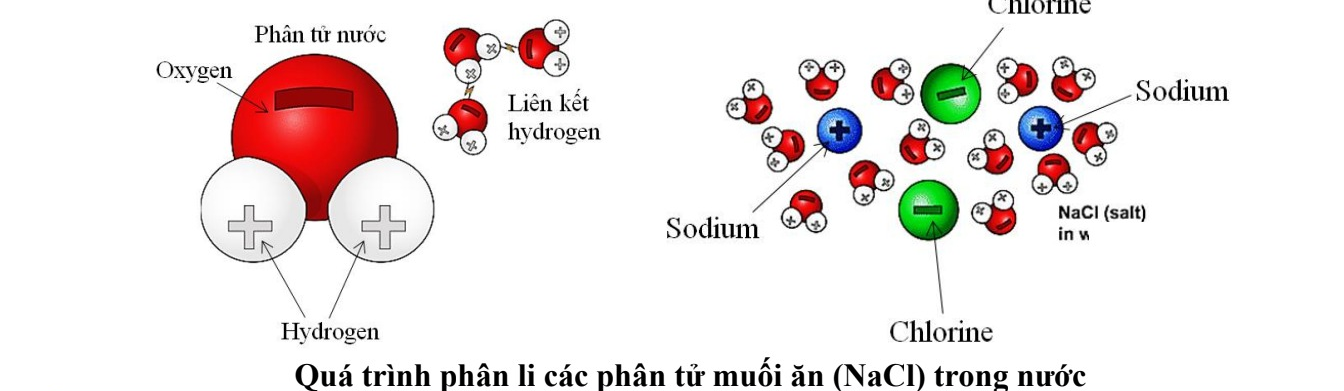
\includegraphics[width=12cm]{images_crop_hoa11_de03/cau4_p2_phan_li_nacl.png}
\end{center}
\choiceTF
{Các phân tử nước kéo các ion sodium và ion chloride ra xa nhau, phá vỡ liên kết ion giữa hai ion sodium và ion chloride.}
{Sau khi các hợp chất muối được tách ra, các ion sodium và ion chloride được bao quanh bởi các phân tử nước. Lúc này, muối sẽ bị hòa tan, tạo thành dung dịch đồng nhất (dung dịch chất dẫn điện).}
{Đầu âm của các phân tử nước bị thu hút bởi các ion chloride tích điện dương, còn đầu dương của các phân tử nước bị thu hút bởi các ion sodium tích điện âm.}
{Sự điện li của $\ce{NaCl}$ trong nước có thể được biểu diễn bằng phương trình điện li như sau: $\ce{NaCl + (a+b)H2O -> Na+.aH2O + Cl-.bH2O}$.}
\loigiai{}
\end{ex}

\bigskip
\noindent
\textbf{PHẦN III (1,5 điểm -- 6 câu): Câu trắc nghiệm yêu cầu trả lời ngắn.}\\
\textit{Thí sinh trả lời từ câu 1 đến câu 6.}

\begin{ex}
Độ pH của da thường từ $4{,}5 - 5{,}5$, có tính Acid nhẹ. Điều này giúp da của chúng ta chống lại vi khuẩn trên bề mặt. Đối với da đầu, độ pH của da đầu thường từ $4 - 7$. Sản phẩm dành cho tóc dầu sẽ có độ pH cao hơn $5{,}5$, chứa chất tẩy rửa mạnh giúp loại bỏ chất dầu nhờn trên da đầu. Bên cạnh đó, nếu bạn thường xuyên uốn nhuộm thì những dòng sản phẩm dành cho tóc hư tổn với khả năng bổ sung tính Acid giúp cân bằng độ pH trên da đầu và tóc sẽ rất hữu ích.
\begin{center}
	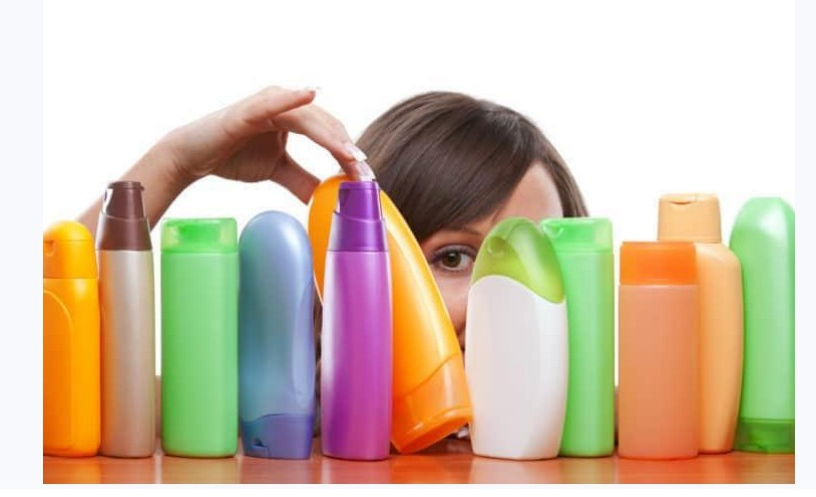
\includegraphics[width=6.5cm]{images_crop_hoa11_de03/cau1_p3_dau_goi.png}
\end{center}
Một loại dầu gội đầu có nồng độ ion $\ce{OH-}$ là $10^{-5{,}17}\text{ mol/L}$. Tính pH của loại dầu gội nói trên (kết quả làm tròn đến hai chữ số phần thập phân).

\vspace{1.2cm}

\end{ex}

\begin{ex}
\textbf{(SBT - KNTT)} Aspirin là một loại thuốc có thành phần chính là acetylsalicylic acid. Nếu hoà tan thuốc này vào nước, người ta xác định được pH của dung dịch tạo thành là $2{,}8$. Nồng độ $\ce{OH-}$ của dung dịch tạo thành là $10^x$. Xác định $x$?

\vspace{1.2cm}

\end{ex}

\begin{ex}
\textbf{[CD - SGK]} Chuẩn độ dung dịch $\ce{NaOH}$ chưa biết chính xác nồng độ (biết nồng độ trong khoảng gần với $0{,}1\text{ M}$) bằng dung dịch chuẩn $\ce{HCl}\ 0{,}1\text{ M}$ với chất chỉ thị phenolphthalein hết $10\text{ mL}$. Giả sử khi kết thúc chuẩn độ, thể tích dung dịch $\ce{NaOH}$ (tính trung bình sau 3 lần chuẩn độ) đã sử dụng ở burette là $10{,}27\text{ mL}$. Nồng độ của dung dịch $\ce{NaOH}$ là $x\text{ (M)}$. Xác định giá trị của $x$ (kết quả làm tròn đến hàng phần mười).

\vspace{1.2cm}

\end{ex}

\begin{ex}
Cần bao nhiêu gam $\ce{NaOH}$ để pha chế $250{,}0\text{ mL}$ dung dịch có $\text{pH} = 12$?

\vspace{1.2cm}

\end{ex}

\begin{ex}
\textbf{[CD - SBT]} Xét phản ứng: $\ce{H2(g) + I2(g) <=> 2HI(g)}$. Một hỗn hợp phản ứng chứa trong bình dung tích $3{,}67\text{ lít}$ ở một nhiệt độ xác định, ban đầu chứa $0{,}763\text{ gam } \ce{H2}$ và $96{,}6\text{ gam } \ce{I2}$. Ở trạng thái cân bằng, bình chứa $90{,}4\text{ gam } \ce{HI}$. Tính hằng số cân bằng ($K_C$) cho phản ứng ở nhiệt độ này (làm tròn kết quả đến phần nguyên).

\vspace{1.2cm}

\end{ex}

\begin{ex}
Trong công nghiệp, hydrogen được sản xuất từ phản ứng:
\[\ce{CH4(g) + H2O(g) <=> 3H2(g) + CO(g)}\]
Tính hằng số cân bằng $K_C$ của phản ứng trên ở $760^\circ\text{C}$. Biết ở nhiệt độ này, tất cả các chất đều ở thể khí và nồng độ mol của $\ce{CH4, H2O, H2}$ và $\ce{CO}$ ở trạng thái cân bằng lần lượt là $0{,}126\text{ M}$; $0{,}242\text{ M}$; $1{,}150\text{ M}$ và $0{,}126\text{ M}$ (làm tròn kết quả đến hàng phần trăm).

\vspace{1.2cm}

\end{ex}

\bigskip
\noindent
\textbf{PHẦN IV: Tự luận}\\
\textit{Học sinh giải chi tiết các câu hỏi sau vào giấy làm bài.}

\begin{ex}
\textbf{[CD - SBT]} Điền từ ngữ thích hợp vào chỗ trống trong mỗi phát biểu sau:\\
a) Quá trình phân li của các chất khi tan trong nước thành các ion được gọi là .....(1)..... Chất điện li là chất khi tan trong nước phân li thành các .....(2)..... .....(3)..... là chất khi tan trong nước không phân li thành các ion.\\
b) Theo thuyết Brønsted -- Lowry, .....(1)..... là những chất có khả năng cho $\ce{H+}$, .....(2)..... là những chất có khả năng nhận $\ce{H+}$. Acid mạnh và base mạnh phân li .....(3)..... trong nước; acid yếu và base yếu phân li .....(4)..... trong nước.

\vspace{2.5cm}

\end{ex}

\begin{ex}
\textbf{(SBT - KNTT)}\\
a) $\ce{CH3COOH}$ (có trong giấm ăn) là một acid yếu. Tính pH của dung dịch $\ce{CH3COOH}\ 0{,}1\text{ M}$ (biết hằng số cân bằng của sự phân li $\ce{CH3COOH}$ là $1{,}8 \cdot 10^{-5}$, bỏ qua sự phân li của nước).\\
b) Trong dung dịch nước ion $\ce{CH3COO-}$ nhận proton của nước. Viết phương trình thuỷ phân và cho biết môi trường của dung dịch $\ce{CH3COONa}$.\\
c) Cho $10\text{ mL}$ dung dịch $\ce{NaOH}\ 0{,}1\text{ M}$ vào $10\text{ mL}$ dung dịch $\ce{CH3COOH}\ 0{,}2\text{ M}$ thu được $20\text{ mL}$ dung dịch A. Tính pH của dung dịch A.

\vspace{3.5cm}

\end{ex}

\begin{center}
\textbf{--------- HẾT ---------}
\end{center}

\end{document}
